\documentclass[12pt,a4paper]{article}
\usepackage[utf8]{inputenc}
\usepackage[francais]{babel}
\usepackage[T1]{fontenc}
\usepackage{amsmath}
\usepackage{amsfonts}
\usepackage{amssymb}
\usepackage{graphicx}
\usepackage{enumitem}
\usepackage{eurosym}
\usepackage[a4paper,left=2cm,right=2cm,top=2cm,bottom=2cm]{geometry}
\usepackage{hyperref}
\usepackage{gensymb}

\usepackage{listings,color}

\definecolor{verbgray}{gray}{0.9}


\setlength{\parskip}{1ex plus 0.5ex minus 0.2ex}
\newcommand{\hsp}{\hspace{20pt}}
\newcommand{\HRule}{\rule{\linewidth}{0.5mm}}

\renewcommand{\thesection}{\Alph{section}}

\begin{document}


\begin{titlepage}
  \begin{sffamily}
  \begin{center}
\begin{figure}

\end{figure}

    \fbox{\textsc{\LARGE Projet bibliographique}}\\[2.5cm]

    \textsc{\Large Rapport final}\\[1.5cm]

    \HRule \\[0.4cm]
    { \huge \bfseries Détection automatique des Nématodes \\[0.4cm] }
 \HRule \\[1.5cm]
 
 \centering{

\includegraphics[scale=1]{logo.png} 
}\\[8cm]


        \begin{flushleft}
	Félix BOUTERAA 
	Abdelwali BLADI \\
	Mohamed OULAAFFART \\
	02/01/2018 \\
	\end{flushleft}  
    
    \begin{flushright}
Tuteur de projet : M. STIENNE
\end{flushright}  

  \end{center}
  \end{sffamily}
\end{titlepage}

\newpage

\tableofcontents

\newpage

\listoffigures

\newpage
\section*{Introduction}
\addcontentsline{toc}{section}{Introduction}
 Les poissons peuvent être infestés par de nombreux parasites incluant les protozoaires, les trématodes, les nématodes et les cestodes Contracaecum, Hysterothylacium
et Pseudoterranova. Les larves de deux espèces de la famille des nématodes Anisakidae. Ces parasites constituent un danger pour la santé publique. En effet,  Ils peuvent entraîner des
pathologies digestives (anisakidose) et allergiques chez
l’Homme. Le nombre de cas d’anisakidose pourrait
augmenter de façon significative au cours des prochaines
années suite à la consommation accrue de produits marinés
ou crus, au non-respect de la réglementation européenne
et au manque de perception du risque (pas de congélation
du produit avant consommation cru) par le consommateur.\\
 Par conséquent et afin de maitriser le risque lié à la présence de ces parasites,
les réglementations européennes (CE 852/2004, CE 853/2004,
CE 854/2004, CE 2074/2005, CE 1276/2011) imposent :
\begin{enumerate}
\item La nécessité d’un contrôle visuel: les produits manifestement parasités ne doivent
pas être missur le marché
 \item Une congélation assainissante obligatoire
(-20 \degree C pendant 24h ou -35 \degree C pendant 15h en tous points du produit)
pour les produits devant être consommés crus ou pratiquement crus
et pour les produits devant subir un traitement de fumage à froid(T < 60 \degree C) et pour les produits marinés et/ou salés si le traitement est insuffisant pour tuer les parasites viables.
\end{enumerate}

\newpage

\section {Les  méthode  non-destructrices de détection des parasites dans les filets de poissons}
\subsection{La table de mirage}
La méthode utilisé dans la majorité des cas pour déterminer la présence de parasite est le mirage qui implique l’inspection de chaque filet à travers une surface illuminée translucide. Cette méthode est limitée parce qu’elle ne peut pas détecter les parasites enkystés à une profondeur supérieure à 6 mm dans le muscle du poisson. Également, elle demeure très fatigante pour l'œil de l'opérateur. Mais son avantage reste le coût du moment qu'elle ne nécessite la mise en place d'un dispositif quelconque.

\begin{figure}[!h]
   \center
   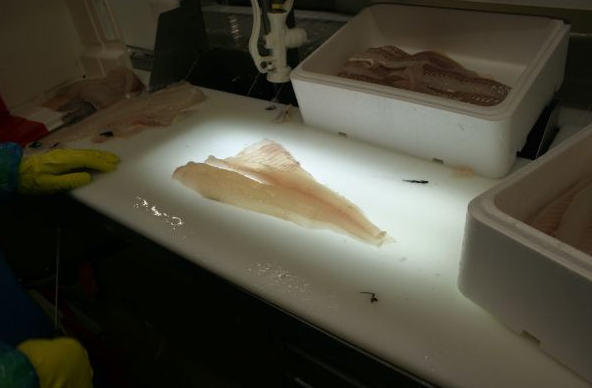
\includegraphics[scale=0.5]{Table_mirage.png}
   \caption {Détection des larves d'Anisakidés en industrie sur table de mirage classique.}
\end{figure}

\subsection{Méthode du mirage au laser}

De nombreuses alternatives ont été tentées pour détecter les parasites dans les filets essentiellement  par exemple le mirage au laser.
Ou qu’on peut appeler par balayage en laser , c’est une technique ou on éclaire le poisson en défilement par un petit impact laser  qui le balaye transversalement a très grande vitesse , cela permet de capter les variations de la luminance qui se produit lorsque le laser rencontre un défaut ou un parasite .
\subsection{Méthode des rayons X}
La Radiographie est aussi utiliser dans la détection de parasites, commençant déjà par connaitre la méthode de rayon X.

Sont des ondes électromagnétiques de très courtes longueurs d’ondes entre (0.1 pm et 1000pm) .Ces rayons X se propagent en ligne droite et à la vitesse de la lumière dans le vide.
Le résultat recueillit est des modulations d’intensité du faisceau sous forme d’image sur un récepteur approprié. Et on peut aussi sous le mémé principe obtenir des résultats en utilisant d’autres particules que le photons comme la neutronographie.

\subsection{Méthode ultrasons}

Les ultrasons sont des vibrations mécaniques prenant naissance et se propageant dans tous le support matériel présentant une certaine élasticité.
Les ultrasons correspondent à des fréquences oscillatoires supérieure à la limites d’audibilité humaine et s’étendant dans une large gamme allant de 15kilohertz à plus de 100 MHz.
Cette méthode et une méthode non destructives car les fréquences correspondent pour les matières à des longueurs d’ondes ultrasonore de l’ordre du millimètre ce qui permet de détecter les petits défauts ainsi les parasites. 

\subsection{Méthode éléctromagnétique}

L’une des méthodes que utilisé pour la détection des parasites et  « la méthode électromagnétique », cette méthode consiste sur la reconnaissance de signal, les parasites sont détectés  par des variations du champ électromagnétique autour du parasite dans la chair du poisson.
Pour cela une expérience était réaliser afin de connaitre la puissance de cette méthode, cette expérience était faite sur du cabillaud du Pacifique, cette expérience a permis de remarquer que la différence dans la taille et la forme du pic correspondant au poisson contaminé est observée selon la taille du parasite, son orientation et sa position dans le filet, le résultat nous as donc permis  de conclure que les parasites sont détectable grâce à cette méthode. Un faible courant électrique est envoyé à travers un filet parasité et le champ magnétique est enregistré par un magnétomètre SQUID. Les résultats indiquent une détection potentielle efficace à l'aide de l'appareil.
Cette méthode est donc innovante et très pratique et permet d’aller plus loin que la méthode de mirage en profondeur



\subsection{Imagerie domaine du visible}


Cette technique donne une image tridimensionnelle de l'échantillon, à la fois spatiale et spectrale. Cela signifie qu'en chaque point de la surface de l'échantillon, un spectre est enregistré. La mise en œuvre de la technique avec la source de lumière d'un côté de l'échantillon et l'unité de détection de l'autre côté garantit que le spectre représente non seulement la surface mais aussi l'intérieur de l'échantillon.
Typiquement, la région de longueur d'onde utilisée représente la partie visible (VIS, 400-700 nm) et proche infrarouge (NIR, 700-1100 nm) du spectre de la lumière.
Une fois les images enregistrés, il est nécessaire d'entraîner un algorithme à reconnaître les parasites et autres composantes de la peau du filet.
Pour cela, il est nécessaire de repérer les différentes longueur d'onde liés aux différentes composantes du filet.


\subsection{Proche infrarouge}

On peut se baser sur un spectromètre proche infrarouge qui mesure la quantité d'eau, de sucre, d'amidon, de graisse et de protéines présents dans les filets de poisson. Le système analyse plusieurs centimètres sous la surface extérieure des aliments - ce qui signifie qu'il peut détecter des éléments non visibleà l'oeil, sous la surface du poisson.


La transmittance est la fraction absorbé par le filet de poisson. La réflectance est la lumière absorbée par l'échantillon.
Pour les deux méthodes, la gamme de longueur d'onde est un facteur important. Par exemple, une plage à ondes courtes (850 - 1050 nm) donne une bonne pénétration de l'échantillon avec la transmission.


\newpage
\section {Les  méthode destructrices de détection des parasites dans les filets de poissons :}
\subsection{Méthode des rayons UV}
La méthode utilisant les rayons UV pour la détection des parasites dans les poissons était l’objet de plusieurs expériences.\\
De prime abord il convient de mettre en exergue les résultats d’une étude, sur laquelle se base le présent chapitre, faite par le laboratoire UK National Reference Laboratory sous le thème « Detection of Anisakidae larvae in fish fillets using ultraviolet transillumination (UVT) ». \\
En effet, les échantillons de poissons utilisé durant l’expérience peuvent être reçus sous forme de poisson entier ou sous forme de filets ou de tissus pré-préparés. Après les échantillons sont numérotés et ceux qui n’ont pas étaient traités sont immédiatement conservés dans un réfrigérateur pour un maximum de 48 heures. Durant l’expérience,  les filets sont traités sur une  table UV transilluminateur et examinés en utilisant la lumière UV.\\
Les larves d'Anisakidae sont fluorescentes sous forme de taches blanches ou de vers individuels (Comme montré dans l'image N..). Les larves peuvent être, ainsi, enlevées par les ouvriers.
\begin{figure}[!h]
   \center
   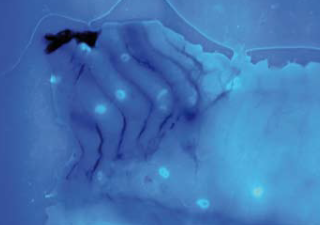
\includegraphics[scale=0.5]{UV.png}
   \caption {Anisakis encapsulé dans un filet de poisson, sous illumination avec une source de lumière ultraviolette. Les parasites individuels apparaissent sous forme d'inclusions lumineuses / fluorescentes dans la chair (image de Wootten et Bron, 2008). [Réf 2]}
\end{figure}
Il est à préciser que les rayons sont dommageables pour les yeux d’où la nécessite d’assurer la protection appropriée et prendre les mesures et précautions adéquates. \\
Par ailleurs, une autre étude a été effectué par Karl, H. Leinemann, en 1993 et publiée sous le thèmes «  fast and quantitative detection method for nematodes in fish fillets and fishery products » vise à trouver une alternative pour la technique de mirage, et ce, afin d’améliorer le taux de détection des nématodes. En effet, L'efficacité de la technique de mirage est limitée par la faible pénétration de la lumière blanche dans le muscle du poisson. \\
Les résultats de cette étude montrent que le taux des parasites détectés sont compris entre 52\% et 98\%, selon l’échantillon utilisé du poisson. \\
Par ailleurs, une expérience faite par « Gaetano Vitale Celano, Antonello Paparella, Armida Fransvea, Claudia Balzaretti, and Giuseppe Celano» dont les résultats les conditions et les résultats sont détaillées dans cette partie.\\
En effet, l’expérience a été effectuée sur 23 échantillons de poissons appartenant à sept espèces différentes qui sont illustrés dans le tableau de la figure N \\
\begin{figure}[!h]
   \center
   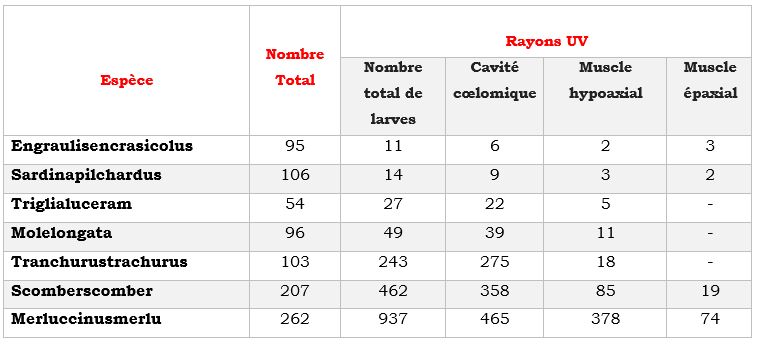
\includegraphics[scale=0.5]{Tableau01.png}
   \caption {Répartition des larves d'anisakidae dans différentes régions anatomiques de sept espèces de poissons). [Réf 2]}
\end{figure}

Pour la transillumination UV a été effectuée comme suit: 
\begin{itemize}
\item   solution saline (1: 5 w / v) à 30 \degree C a été ajouté à des échantillons de poisson, qui ont ensuite été homogénéisés dans un stomacher pendant 1 à 2 minutes.
\item l'homogénat a été pressé à couche mince de 5 mm et examiné sous lumière UV à 366 nm dans une pièce sombre. Dans de telles conditions de fonctionnement, les larves restent intactes.
\end{itemize} 
Les résultat obtenus grâce à ces deux méthodes : l’observation directe et la transillumination UV sont consignés dans le tableau ci-dessous.\\  
L'analyse des résultats obtenus comme suit :
\begin{itemize}
\item En Transillumination UV, les larves d'une taille de 1 à 3 cm étaient fluorescents blanc pourrait être facilement différencié des fibres musculaires des poissons.
\item  	Dans un grand nombre d'échantillons les nématodes se déplaçaient activement et étaient clairement visibles sous la transillumination UV.
 \item	Le tableau montre la répartition des échantillons positifs dans la différente région anatomique des sept espèces de poissons, analysé par la méthode UV. Les données suggèrent que le degré d'infestation de la cavité cœlomique n'est pas en corrélation avec le degré d'infestation et localisation dans le muscle, mais peut être liée à des espèces de poissons. Dans cette étude, la récupération des tissus musculaires nettement plus élevé dans les échantillons analysés par transillumination UV. La même méthode peut également être utilisée pour distinguer les larves viables des larves mortes en colorant les larves avec plusieurs colorants ou en ajoutant du chlorure de tétrazolium . 
\end{itemize} 
\newpage


\newpage
\section*{Webographie}
\addcontentsline{toc}{section}{Bibliographie}

\begin{enumerate}
		\item https://www.cefas.co.uk/anisakis/methods/nrl001-ultraviolet-transillumination/
	\item https://www.cefas.co.uk/media/180326/uk\_anisakis\_nrl\_final\_report\_2014-2015.
	\item http://www.vliz.be/imisdocs/publications/70843.pdf.
	\item http://www.ijbbb.org/papers/240-S037.pdf
	\item \item http://bulletinepidemiologique.mag.anses.fr/sites/default/files/BEP-mg-BE55-Art3.pdf
	\item http://www.fish-parasites.com/accueil/actions/item/172-developing-optimizing-innovative-approaches-for-the-online-detection-of-anisakidae-larvae
	\item \href{https://www.fcm.fraunhofer.de/en/beispiele11/nie-mehr-die-katze-im-sack-kaufen.html}{https://www.fcm.fraunhofer.de/en/beispiele11/nie-mehr-die-katze-im-sack-kaufen.html}
	\item \href{https://www.fossanalytics.com/fr-fr/news-articles/technologies/nir}{https://www.fossanalytics.com/fr-fr/news-articles/technologies/nir}
	\href{https://brage.bibsys.no/xmlui/bitstream/handle/11250/282809/Rapport\%2B19-2003\%2BImaging\%2BSpectroscopy.pdf?sequence=3}{https://brage.bibsys.no/xmlui/bitstream/handle/11250/282809/Rapport\%2B19-2003\%2BImaging\%2BSpectroscopy.pdf?sequence=3}
	\item Livre : Contrôle non destructif (CND)
	
	\item http://bibliomer.ifremer.fr/consult.php?ID=1994-0301
	
	\item http://bibliomer.ifremer.fr/consult.php?ID=1996-0509
	
	\item http://bibliomer.ifremer.fr/consult.php?ID=2000-0884

	
\end{enumerate}

\end{document}